\chapter{FUENTE DE DATOS Y PREPARACIÓN}
\label{cap:dataset}
\section{Origen y alcance}
La fuente seleccionada es Wikipedia Recent Changes, publicada por Wikimedia EventStreams. El consumidor utiliza el endpoint \url{https://stream.wikimedia.org/v2/stream/recentchange} y procesa eventos SSE con contenido JSON. El repositorio configura las wikis mediante \codigo{WIKIS}, cuyo valor predeterminado es \codigo{enwiki,eswiki} \cite{repo}.

EventStreams permite solicitar un inicio temporal con \codigo{since} y retomar el consumo con \codigo{Last-Event-ID}. La documentación oficial advierte que el historial es finito y depende del stream; por tanto, el respaldo externo no debe tratarse como archivo permanente. Los eventos de prueba con \codigo{meta.domain=canary} se descartan \cite{wikimedia}.

El sistema conserva metadatos de cambios, identificadores, comentarios y tamaños; no descarga el texto completo de todas las revisiones. En consecuencia, el volumen neto expresa variación de bytes y las reversiones se infieren de comentarios. El análisis no ofrece una clasificación semántica del contenido.

\section{Estructura semiestructurada}
Los documentos comparten datos de la wiki, el editor, la página y el momento del evento, pero presentan campos diferentes según su tipo. La tabla~\ref{tab:tipos} resume los cuatro tipos aceptados por la limpieza.

\begin{tabla}
\begin{tabularx}{\textwidth}{P{2.1cm}YY}
\toprule
Tipo & Significado & Campos específicos utilizados \\
\midrule
\codigo{edit} & Modificación de una página existente. & \codigo{length}, \codigo{revision}, comentario y marca \codigo{minor}. \\
\codigo{new} & Creación de una página. & Tamaño inicial y revisión nueva. \\
\codigo{categorize} & Cambio de pertenencia a una categoría. & Título de categoría y enlace a la página en el comentario. \\
\codigo{log} & Acción de registro o administración. & \codigo{log_type}, \codigo{log_action}, \codigo{log_params}. \\
\bottomrule
\end{tabularx}
\caption{Tipos de evento admitidos por el pipeline.}\label{tab:tipos}
\end{tabla}

Los campos comunes requeridos por la validación Python son \codigo{type}, \codigo{wiki}, \codigo{title}, \codigo{namespace}, \codigo{user} y \codigo{timestamp}; además, \codigo{meta} debe contener un identificador y una fecha interpretables. Los objetos anidados y las variantes de \codigo{log_params} justifican su naturaleza semiestructurada.

\par\noindent\begin{minipage}{\linewidth}
\begin{lstlisting}[caption={Ejemplo didáctico de un evento de edición; no es una medición.}]
{
  "meta": {"id": "ejemplo-001", "dt": "2026-11-17T10:04:00Z"},
  "type": "edit", "wiki": "eswiki", "title": "Pagina de ejemplo",
  "namespace": 0, "user": "EditorEjemplo", "timestamp": 1794909840,
  "bot": false, "comment": "",
  "length": {"old": 1000, "new": 1250}
}
\end{lstlisting}
\end{minipage}\par

\section{Selección empírica y volumen}
La captura exploratoria del 31 de octubre registró 4\,915 eventos válidos durante 134 segundos, distribuidos entre 93 wikis, 607 usuarios y 2\,758 páginas. Sus tipos fueron 2\,323 categorizaciones, 2\,105 ediciones, 260 creaciones y 227 registros \cite{dataset}. La tasa observada sobre esa muestra fue:
\[
\frac{4915}{134}=36.68\ \text{eventos/s}.
\]
Esta medición corresponde al stream multilingüe de exploración. No representa la tasa del pipeline final filtrado a dos wikis y no debe extrapolarse como su capacidad sostenida.

\begin{figure}[htbp]
\centering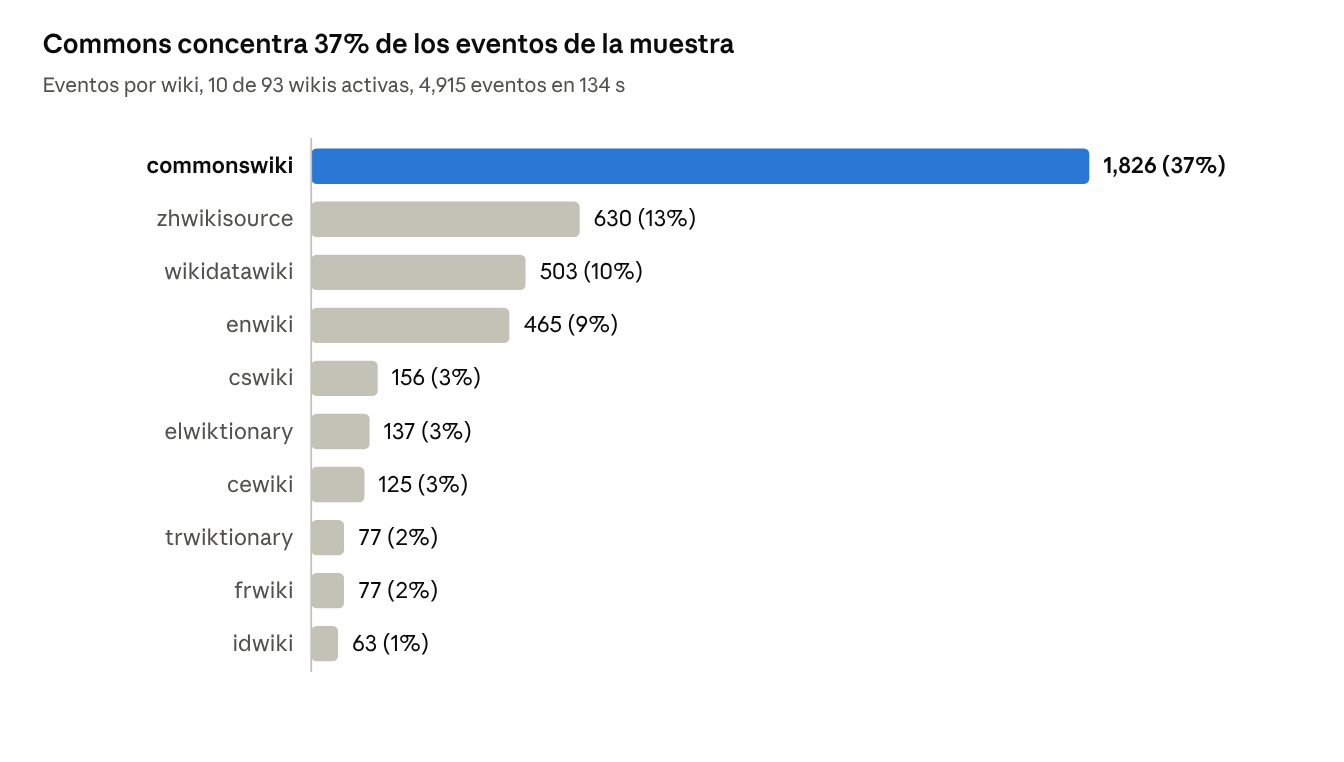
\includegraphics[width=0.93\textwidth]{eventos-por-wiki.png}
\caption{Distribución por wiki en la captura exploratoria multilingüe.}
\fuente{imagen y muestra del 31 de octubre incluidas en \ruta{docs/justificacion-dataset.md}}
\end{figure}

Para el alcance final, la bitácora registra ventanas de 16\,442 y 15\,402 eventos en dos horas del 31 de octubre. Más adelante se documentaron millones de eventos acumulados; sin embargo, ese historial fue recortado durante la migración del 17 de noviembre. Después de la reconstrucción se reportaron 206\,762 eventos desde las 01:00 UTC de ese día, equivalentes a 4.14 veces el mínimo requerido \cite{bitacora}. Es una cifra documentada de ese corte y no una consulta en vivo realizada durante la redacción.

\section{Validación, deduplicación y enriquecimiento}
La función \codigo{validate} devuelve un motivo explícito cuando un documento incumple las reglas. Se comprueba la presencia de campos, los tipos de texto, el \codigo{namespace} entero, el booleano \codigo{bot}, la fecha, la estructura de \codigo{length} y ciertos parámetros de registro. La validación de \codigo{timestamp} exige su presencia; la asignación temporal del procesamiento utiliza \codigo{meta.dt}.

La limpieza escribe dos archivos comprimidos: eventos aceptados y rechazados con su motivo. Un conjunto de identificadores evita duplicados dentro del archivo. Los documentos aceptados reciben \codigo{_id=meta.id} y un bloque \codigo{derived}. Los campos originales se mantienen salvo la normalización de claves que aplica la carga documental.

\begin{tabla}
\begin{tabularx}{\textwidth}{P{4.0cm}Y}
\toprule
Campo derivado & Uso \\
\midrule
\codigo{event_time}, \codigo{event_dt} & Momento normalizado en UTC; texto ISO y fecha BSON respectivamente. \\
\codigo{date}, \codigo{hour}, \codigo{minute} & Construcción de ventanas y series temporales. \\
\codigo{user_type} & Clasificación en bot, temporal, IP o registrado. \\
\codigo{page_key} & Identidad \codigo{wiki:title} para evitar mezclar páginas de wikis distintas. \\
\codigo{delta_bytes} & Diferencia entre tamaño nuevo y anterior en \codigo{edit} y \codigo{new}. \\
\codigo{revert_target}, \codigo{message_target} & Destinatarios inferidos de reversiones y mensajes. \\
Campos de categorías y registros & Página categorizada, acción, bloqueo, agradecimiento, traslado o archivo. \\
\bottomrule
\end{tabularx}
\caption{Enriquecimiento de los documentos aceptados.}
\end{tabla}

\subsection{Clasificación de editores}
Se considera bot a un evento marcado como tal, a una cuenta cuyo nombre satisface la expresión regular de bot o a una cuenta incluida en \codigo{KNOWN_BOTS}, como Automoderador. Las cuentas que comienzan con \texttt{\textasciitilde} se clasifican como temporales; los nombres que representan una IP se identifican con \codigo{ipaddress}; los restantes se consideran registrados. Es una regla práctica cuya precisión no fue medida con un conjunto de etiquetas independiente.

\subsection{Detección de reversiones y relaciones}
Una reversión requiere un enlace a contribuciones de otro editor y palabras de reversión en inglés o español. Se excluyen avisos con \codigo{Warning}, \codigo{Reporting}, restauraciones con \codigo{Restored} y autorreversiones. Los mensajes se infieren de ediciones en el espacio de discusión de usuarios, \codigo{namespace=3}. La categorización combina el enlace a la página con frases de adición o eliminación.

Estas reglas ofrecen evidencia de actividad de revisión, pero pueden omitir formatos de comentario no contemplados. Un \codigo{revert_target} es un resultado heurístico, no una etiqueta definitiva de vandalismo.

\section{Calidad y límites de cobertura}
La calidad se calcula como eventos válidos únicos divididos entre entradas leídas por la limpieza. Los duplicados se contabilizan aparte, pero permanecen en el denominador; por ello pueden reducir el porcentaje sin ser rechazos. Los registros descartados antes de formar el archivo, como otras wikis o eventos sin fecha interpretable durante la extracción, quedan fuera de ese indicador.

Un resultado de 100\,\% significa que todas las entradas consideradas pasaron las reglas y la deduplicación. No demuestra cobertura total del stream, ausencia de sesgo, exactitud semántica ni disponibilidad continua. La cobertura se administra por separado con tramos persistidos y recuperación de ventanas.
